\chapter{Описание математической модели движения недеформируемого водного робота с острой кромкой}\label{ch:ch6}

В данной главе представлены результаты разработки математической модели движения недеформируемого водного робота с острой кромкой в жидкости. Описана методика определения гидродинамических сил и моментов, действующих на тело. На основании полученных уравнений движения проведено моделирование и получены траектории, которые можно использовать как  базовые маневры.

\section{Уравнения движения}

\subsection{Подходы к построению математической модели}


%В представленном исследовании мы изучаем управляемую динамику надводного робота. Данный робот состоит из корпуса в форме крылового профиля NACA0040, управляющей электроники и ротора, за счет крутильных колебаний которого робот приводится в движение.

Траекторное управление движением данного робота оказывается крайне нетривиальной задачей. Так для полного математического описания динамики требуется совместное численное решение уравнений динамики твердого тела и уравнений Навье-Стокса. Это, в частности, не позволяет вычислять управляющие воздействия в реальном времени. Кроме того, в рамках математической модели крайне затруднительно учесть влияние границ, как свободных, так неподвижных.

В связи с этим в данной работе мы рассмотрим \textit{упрощенную конечномерную модель, качественно описывающую управляемое плоскопараллельное движение рассматриваемого робота в неограниченном объеме жидкости}. В данной модели не учитывается ряд факторов, возникающих при движении робота: ошибки в измерении скорости движение робота, его положения и ориентации, образование волн, влияние границ бассейна, наличие фоновых течений, качка и т. п.

На основе предложенной математической модели мы строим управления (\textit{гейты}\footnote{Под \textit{гейтом}  понимается закон вращения ротора, обеспечивающий некоторый простой маневр, например, направленное движение или разворот.}), позволяющие осуществлять простейшие маневры, комбинируя которые можно реализовать сложное движение робота вблизи заданной траектории. %Отметим, что в силу ряда допущений математической модели гейты, полученные на ее основе, могут обеспечивать лишь качественное согласование с экспериментом. Их уточнение является задачей дальнейших экспериментальных исследований.

В данной работе для описания движения мы воспользуемся уравнениями Ньютона-Эйлера при дополнительном предположении, что силы и момент сил, действующие на тело, зависят только от его скоростей и ускорений. Так в подвижных осях, жестко связанных с телом, уравнения движения имеют вид:
\begin{gather}
\begin{gathered}
m \dot{v}_1 = m v_2 \omega + f_1 (v_1,\, v_2,\, \omega,\, \dot{v}_1,\, \dot{v}_2,\, \dot \omega),\quad m \dot{v}_2 = -m v_1 \omega + f_2 (v_1,\, v_2,\, \omega,\, \dot{v}_1,\, \dot{v}_2,\, \dot \omega),\\
I \dot{\omega} = g (v_1,\, v_2,\, \omega,\, \dot{v}_1,\, \dot{v}_2,\, \dot \omega),
\end{gathered}\label{eq.NE}
\end{gather}
где $m$, $I$ --- масса и момент инерции робота соответственно, $f_1$, $f_2$ --- проекции силы реакции жидкости на подвижные оси, связанные с телом, $g$ --- момент силы реакции жидкости. 

Если жидкость идеальная и циркуляция вокруг тела отсутствует, то гидродинамическое сопротивление описывается только эффектом присоединенных масс, а уравнения \eqref{eq.NE} принимают вид уравнений Кирхгофа для плоскопараллельного движения \cite{Kirchhoff}. При наличии циркуляции вокруг тела дополнительно возникают гироскопические силы (в частности подъемная сила), и уравнения принимают вид уравнений Чаплыгина \cite{Borisov_Mamaev, Chaplygin}. Воспользуемся в данном случае этими соображениями для построения зависимостей для сил $f_1$, $f_2$ и момента $g$, и дополним их квадратичными слагаемыми, описывающими вязкое сопротивление среды.

В данной работе считаем, что вязкое сопротивление зависит от скорости квадратично, а коэффициент сопротивления постоянный. Такой выбор обусловлен тем, что движение робота совершается при числах Рейнольдса $Re \sim 1000$, и в аналогичной ситуации сопротивление кругового цилиндра зависит от скорости также квадратично с почти постоянным коэффициентом сопротивления \cite{Schlichting}.

Построенные таким образом выражения для сил $f_1$, $f_2$ и момента $g$ будут содержать коэффициенты присоединенных масс, присоединенного момента инерции и коэффициенты вязкого сопротивления. Для их определения мы воспользуемся моделированием движения робота на основе совместного численного решения уравнений движения тела и уравнений Навье-Стокса как по некоторым модельным траекториям, так и по траекториям, полученным экспериментально.

%В общем случае можно указать три общепринятых подхода к построению зависимостей $f_1$, $f_2$, $g$.	
	
%\textbf{На основе физического эксперимента.} 
	
%В этом случае принимаются некоторые (весьма произвольные) предположения о зависимости сил $f_1$, $f_2$ и момента $g$ от скоростей и ускорений. Коэффициенты модели подбираются таким образом, чтобы решение уравнений \eqref{eq.NE} наилучшим образом описывало экспериментальные данные. 
	
%Отметим, что построенные таким способом выражения для $f_1$, $f_2$ и $g$ могут не иметь физического смыла. По этой причине согласования расчетов и эксперимента удается добиться лишь для небольшого диапазона движений, а сама математическая модель оказывается неприменимой для <<чернового>> проектирования.
	

\subsection{Общий вид уравнений движения}

%В качестве первого приближения будем строить модель плоскопараллельного движения симметричного крылового профиля в вязкой жидкости. При этом будем пренебрегать влиянием вихревых структур.

%Начнем построение математической модели с анализа уравнений Кирхгофа \cite{Kirchhoff_1869}, описывающих движение твердого тела в идеальной жидкости. При этом будем учитывать вязкое сопротивление и пренебрегать влиянием вихревых структур.

Для описания движения робота введем две системы координат: неподвижную $Oxy$ и подвижную $Cx_1x_2$ жестко связанную с телом (см. рис. \ref{fig.coords}). Будем считать, что ось $Cx_1$ подвижной системы координат совпадает с осью симметрии профиля, а точка $C$ совпадает с центром масс системы <<профиль + ротор>>. Положение подвижной системы координат относительно неподвижной будем задавать с помощью радиус-вектора $\bm r = (x,\, y)$ точки $C$, а ее ориентацию углом $\alpha$ между положительными направлениями осей $Ox$ и $Cx_1$, отсчитываемым от оси $Ox$.

\begin{figure}[h!]
	\centering
	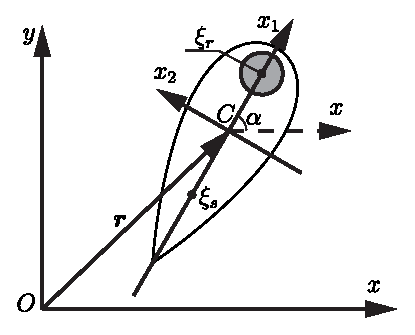
\includegraphics{coords.eps}
	\caption{$Oxy$ --- неподвижная система координат, $Cx_1x_2$ --- подвижная система координат}\label{fig.coords}
\end{figure}

Справедливы следующие кинематические соотношения:
\begin{gather}
\begin{gathered}
\dot{x} = v_1 \cos\alpha - v_2 \sin\alpha,\quad \dot{y} = v_1 \sin\alpha + v_2 \cos\alpha,\quad \dot{\alpha} = \omega,
\end{gathered}\label{eq.kinem}
\end{gather}
где $v_1$, $v_2$ --- проекции вектора поступательной скорости точки $C$ на подвижные оси, $\omega$ --- угловая скорость тела.

Движение твердого тела в идеальной жидкости при нулевой циркуляции описывается уравнениями Кирхгофа \cite{Kirchhoff}. Поскольку эти уравнения учитывают только эффект присоединенных масс и моментов инерции\footnote{Присоединенные массы и моменты инерции --- описывают реакцию среды на ускоренное движение тела и обусловлены распределением давления по поверхности тела.}, их необходимо дополнить слагаемыми, описывающими вязкое трение \cite{Borisov_et_al_2016}:
\begin{gather}
\begin{gathered}
\der{}{t} \pder{T}{v_1} = \omega \pder{T}{v_2} - c_1 v_1 |v_1|,\quad \der{}{t} \pder{T}{v_2} = - \omega \pder{T}{v_1} - c_2 v_2 |v_2|,\\
\der{}{t} \pder{T}{\omega} = v_2 \pder{T}{v_1} - v_1 \pder{T}{v_2} - c_3 \omega |\omega|,
\end{gathered}\label{eq.kirchhoff}
\end{gather}
где $T$ --- кинетическая энергия системы (корпус + ротор + жидкость), $c_1$, $c_2$, $c_3$ --- коэффициенты сопротивления.

Кинетическая энергия системы с точностью до некоторой функции времени имеет вид
\begin{gather}
T = \frac{1}{2}(m + \lambda_{11}) v_1^2 + \frac{1}{2}(m + \lambda_{22}) v_2^2 + \frac{1}{2} (I + \lambda_{33}) \omega^2 + \lambda_{23} v_2\omega + \omega k(t),\label{eq.T}\\
\begin{gathered}
m = m_s + m_r,\quad
I = I_s + m_s \xi_s^2 + I_r + m_r \xi_r^2,\quad k(t) = I_r \Omega(t),
\end{gathered}\notag
\end{gather}
где $m_s$, $I_s$ --- масса и центральный момент инерции корпуса робота, $m_r$, $I_r$ --- масса и центральный момент инерции ротора, $\xi_s$ --- положение центра масс корпуса робота, $\xi_r$ --- положение центра масс ротора, $\Omega(t)$ --- угловая скорость ротора, $\lambda_{11}$, $\lambda_{22}$ --- присоединенные массы, $\lambda_{33}$ --- присоединенный момент инерции, $\lambda_{23}$ --- коэффициент, возникающий вследствие смещения центра давления относительно центра масс.

%Отметим, что слагаемое $\lambda_{23} v_2\omega$ в выражении \eqref{eq.T} возникает вследствие смещения центра давления относительно центра масс. 
Отметим, что в выражении \eqref{eq.T} отсутствует слагаемое с $v_1 \omega$, так как профиль является зеркально симметричным относительно оси $Cx_1$. Кроме того, в силу выбора начала подвижной системы координат выполняется соотношение
\begin{gather*}
m_s \xi_s + m_r \xi_r = 0.
\end{gather*}

\textit{Полная система уравнений рассматриваемой системы может быть записана в следующей форме}:
\begin{subequations}\label{eq.fullEqs}
	\begin{equation}
	\begin{split}\label{eq.dyn}
	(m + \lambda_{11}) \dot{v}_1 = {} & {} (m + \lambda_{22}) v_2 \omega + \lambda_{23}\omega^2 - c_1 v_1 |v_1|,\\
	(m + \lambda_{22}) \dot{v}_2 + \lambda_{23} \dot{\omega} = {} & {} - (m + \lambda_{11}) v_1 \omega - c_2 v_2 |v_2|,\\
	\lambda_{23}\dot{v}_2 + (I + \lambda_{33}) \dot{\omega} = {} & {} (\lambda_{11} - \lambda_{22}) v_1 v_2 - \lambda_{23} v_1\omega - c_3 \omega |\omega| - \dot{k}(t),
	\end{split}
	\end{equation}
	\begin{equation}
	\dot{x} = v_1 \cos\varphi - v_2 \sin\varphi,\quad \dot{y} = v_1 \sin\varphi + v_2 \cos\varphi,\quad \dot{\varphi} = \omega.
	\end{equation}
\end{subequations}

Сравнивая уравнения \eqref{eq.dyn} с уравнениями Ньютона-Эйлера \eqref{eq.NE}, запишем выражения для сил $f_1$, $f_2$ и момента $g$:
\begin{gather}
	\begin{gathered}\label{eq.forceTorque}
		f_1 = - \lambda_{11}\dot{v}_1 + \lambda_{22} v_2 \omega + \lambda_{23}\omega^2 - c_1 v_1 |v_1|, \\
		f_2 = - \lambda_{22} \dot{v}_2 - \lambda_{23} \dot{\omega} - \lambda_{11} v_1 \omega - c_2 v_2 |v_2|,\\
		g = -\lambda_{23}\dot{v}_2 - \lambda_{33} \dot{\omega} + (\lambda_{11} - \lambda_{22}) v_1 v_2 - \lambda_{23} v_1\omega - c_3 \omega |\omega| - \dot{k}(t),
	\end{gathered}
\end{gather}
где коэффициенты $\lambda_{ij}$ и $c_i$ подлежат определению, а $\dot{k}(t)$ --- определяется управляющим воздействием на ротор.

Для определения коэффициентов, входящих в эти выражения, мы воспользуемся подходом, основанным на (численном) решении уравнений Навье-Стокса.

%Выражения \eqref{eq.forceTorque} содержат семь коэффициентов: $\lambda_{11}$, $\lambda_{22}$, $\lambda_{33}$, $\lambda_{23}$, $c_1$, $c_2$, $c_3$. Далее мы рассмотрим два подхода к определению этих коэффициентов.


\subsection{Определение сил и моментов сопротивления с использованием уравнений Навье-Стокса}

%	Для определения коэффициентов в \ref{eq.forceTorque} ...
%	
%	\textbf{\textcolor{red}{Вот тут не понятно... м.б. сюда чать из введения о сложности определения этих коэффициентов, а потом к подходу}}


Движение жидкости, окружающей профиль, будем моделировать на основе уравнений Навье-Стокса. Поскольку область, занятая жидкостью, имеет криволинейные границы, для численного решения уравнений динамики жидкости будем использовать криволинейную ортогональную сетку (см. рис. \ref{fig.mesh}).
\begin{figure}[ht!]
	\centering
	\includegraphics{mesh.eps}
	\caption{Вид расчетной сетки, построенной комплексным методом граничных элементов \cite{Hromadka_Lai_2012}}\label{fig.mesh}
\end{figure}
Уравнения Навье-Стокса, записанные относительно криволинейной системы координат $(\xi,\, \eta)$, связанной с движущимся профилем имеют вид:
\begin{gather}
	\begin{gathered}
		\pder{Du_1}{\xi} + \pder{Du_2}{\eta} = 0,\\
		\begin{split}
			\pder{u_1}{t} + \frac{1}{D^2} \biggl( \pder{D(u_1 - w_1)u_1}{\xi} + & \pder{D(u_2 - w_2)u_1}{\eta} \biggr) = \\
			= - \frac{1}{D\rho} \pder{p}{\xi} + & \frac{\nu}{D^2} \left( \pdder{u_1}{\xi}{2} + \pdder{u_1}{\eta}{2} \right) + \beta_1 + 2 u_2 \omega
		\end{split}\\
		\begin{split}
			\pder{u_2}{t} + \frac{1}{D^2} \biggl( \pder{D(u_1 - w_1)u_2}{\xi} + & \pder{D(u_2 - w_2)u_2}{\eta} \biggr) = \\
			= - \frac{1}{D\rho} \pder{p}{\eta} + & \frac{1}{D^2} \left( \pdder{u_2}{\xi}{2} + \pdder{u_2}{\eta}{2} \right) + \beta_2 - 2 u_1 \omega,
		\end{split}
	\end{gathered}
\end{gather}
где $u_1$, $u_2$ --- проекции вектора скорости жидкости на криволинейные оси, $p$ --- давление, $\rho$ --- плотность жидкости, $\nu$ --- кинематическая вязкость, $w_1=v_1 - \omega x_2(\xi,\, \eta)$, $w_2 = v_2 + \omega x_1(\xi,\, \eta)$ --- компоненты переносной скорости. Коэффициент Ламэ $D$ и члены $\beta_1$, $\beta_2$, возникающие вследствие искривления сеточных линий, имеют вид:
\begin{gather*}
	D = \sqrt{\left( \pder{x_1}{\xi}\right)^2 + \left( \pder{x_2}{\xi}\right)^2  } =\sqrt{\left( \pder{x_1}{\eta}\right)^2 + \left( \pder{x_2}{\eta}\right)^2  },\\
	\begin{split}
		\beta_1 = \frac{\nu}{D^3} \Biggl( u_1\left( \pdder{D}{\xi}{2} + \pdder{D}{\eta}{2} \right) + {} & {} 2 \pder{u_1}{\xi} \pder{D}{\xi} + 2 \pder{u_2}{\xi} \pder{D}{\eta} + \\
		+ {} & {} \frac{2u_2}{D} \pder{D}{\xi} \pder{D}{\eta} - \frac{2u_1}{D} \left( \pder{D}{\eta} \right)^2  \Biggr),
	\end{split}\\
	\begin{split}
		\beta_2 = \frac{\nu}{D^3} \Biggl( u_2\left( \pdder{D}{\xi}{2} + \pdder{D}{\eta}{2} \right) + {} & {} 2 \pder{u_1}{\eta} \pder{D}{\xi} + 2 \pder{u_2}{\eta} \pder{D}{\eta} + \\
		+ {} & {} \frac{2u_1}{D} \pder{D}{\xi} \pder{D}{\eta} - \frac{2u_2}{D} \left( \pder{D}{\xi}\right)^2 \Biggr).
	\end{split}
\end{gather*}

При известных распределениях $u_1$, $u_2$, $p$ cилы $f_1$, $f_2$ и момент $g$, действующие на тело со стороны жидкости, определяются следующими интегралами по контуру $L$ профиля:
\begin{gather}
	\begin{gathered}
		f_1 = \oint_L \left( p \pder{x_2}{\xi} + \frac{\rho \nu}{D} \pder{u_1}{\eta} \pder{x_1}{\xi} \right) d\xi,\\
		f_2 = \oint_L \left( -p \pder{x_1}{\xi} + \frac{\rho \nu}{D} \pder{u_1}{\eta} \pder{x_2}{\xi} \right) d\xi,\\
		g = \oint_L \left( x_1 \left( -p \pder{x_1}{\xi} + \frac{\rho \nu}{D} \pder{u_1}{\eta} \pder{x_2}{\xi} \right) - x_2 \left( p \pder{x_2}{\xi} + \frac{\rho \nu}{D} \pder{u_1}{\eta} \pder{x_1}{\xi} \right) \right) d\xi - \dot{k}(t).
	\end{gathered}\label{eq.fgNS}
\end{gather}

Рассмотрим теперь движение профиля по заданному закону и вычислим зависимости $f_1(t)$, $f_2(t)$ и $g(t)$, пользуясь соотношениями \eqref{eq.fgNS}. Сравнивая их с соотношениями \eqref{eq.forceTorque} мы подберем неизвестные коэффициенты таким образом, чтобы наиболее точно воспроизвести полученные зависимости.

\subsubsection*{Квазистационарное обтекание}

В первом приближении вычислим коэффициенты присоединенных масс, присоединенного момента инерции и коэффициенты сопротивления, используя простейшие движения профиля специального вида. Так для определения коэффициентов $\lambda_{11}$, $c_1$ выберем следующий закон движения:
\begin{gather}
	v_1(t) = V_0 \Sigma_{t_1}(t),\quad v_2(t) \equiv 0,\quad \omega(t) \equiv 0,
\end{gather}
где $\Sigma_{t_1}(t)$ кусочно линейная функция вида (см. рис. \ref{fig.sigma})
\begin{gather}
	\Sigma_{t_1}(t) = \begin{cases}
		t / t_1, & 0 \leqslant t < t_1,\\
		1, & t_1 \leqslant t.
	\end{cases}
\end{gather}

\begin{figure}[ht!]
	\centering
	\includegraphics{speedup.eps}
	\caption{Вид функции $\Sigma_{t_1}(t)$}\label{fig.sigma}
\end{figure}

На промежутке времени $t \in [0,\, t_1]$ тело движется прямолинейно равноускоренно, при этом сопротивление жидкости будет определяться преимущественно распределением давления по контуру профиля (эффект присоединенных масс), а вязкие эффекты будут пренебрежимо малы. Как показывают численные эксперименты, на данном промежутке времени сопротивление определяет только эффектом присоединенных масс. По результатам моделирования движения профиля, на данном промежутке времени вычислим присоединенную массу $\lambda_{11} = |f_1 t_1 / V_0|$.

На промежутке времени $t > t_1$ тело движется равномерно, при этом происходит существенное изменение распределения давления по контуру профиля вследствие вязкого трения, возникает лобовое сопротивление. По результатам моделирования в некоторый момент времени $t_2 > t_1$, когда течение становится квазистационарным, вычислим коэффициент сопротивления $c_1 = |f_1| / V_0^2$.

Законы движения профиля, использованные для определения различных коэффициентов модели, приведены в следующем списке:
\begin{itemize}
	\item[$-$] Коэффициенты $\lambda_{11}$, $c_1$. Скорость $v_1(t) = V_0 \Sigma_{t_1}(t)$, $v_2(t) \equiv 0$, $\omega(t) \equiv 0$. Параметры $V_0 = 0.05$, $t_1 = 0.005$.
	\item[$-$] Коэффициенты $\lambda_{22}$, $c_2$. Скорость $v_2(t) = V_0 \Sigma_{t_1}(t)$, $v_1(t) \equiv 0$, $\omega(t) \equiv 0$. Параметры $V_0 = 0.05$, $t_1 = 0.005$.
	\item[$-$] Коэффициенты $\lambda_{33}$, $c_3$. Скорость $\omega(t) = \Omega_0 \Sigma_{t_1}(t)$, $v_1(t) \equiv 0$, $v_2(t) \equiv 0$. Параметры $\Omega_0 = 1$, $t_1 = 0.1$.
	\item[$-$] Коэффициент $\lambda_{23}$. Скорость $v_2(t) = V_0 \Sigma_{t_1}(t)$, $\omega(t) = \Omega_0 \Sigma_{t_1}(t)$, $v_1(t) \equiv 0$. Параметры $V_0 = 0.05$, $\Omega_0 = 1$.
\end{itemize}

В результате обработки данных численного эксперимента получим следующие значения:
\begin{gather}
	\begin{gathered}
		\lambda_{11} \approx 13.453, \quad \lambda_{22} \approx 88.338,\quad \lambda_{33} \approx 0.391,\quad \lambda_{23} \approx 3.495,\\
		c_1 = 53.973,\quad c_2 = 690.14,\quad c_3 = 0.832.
	\end{gathered}\label{eq.val1m}
\end{gather}

Значения \eqref{eq.val1m} определяют удельные силы $f_1$, $f_2$ и момент $g$ (отнесенные к одному метру), действующие на профиль бесконечной длины. Предложенный экспериментальный образец имеет смоченную часть высотой $0.0335$ м. Выполним коррекцию коэффициентов \eqref{eq.val1m} с учетом данной высоты:
\begin{gather}
	\begin{gathered}
		\lambda_{11} \approx 0.451, \quad \lambda_{22} \approx 2.959,\quad \lambda_{33} \approx 0.0131,\quad \lambda_{23} \approx 0.117,\\
		c_1 = 1.808,\quad c_2 = 23.120,\quad c_3 = 0.0279.
	\end{gathered}\label{eq.coeffs1}
\end{gather}


Отметим, что вычисленные присоединенные массы в высокой точностью совпадают со значениями, полученными классическим путем \cite{Korotkin}:
\begin{gather*}
	\lambda_{ij} = \oint_\Gamma \varphi_i \pder{\varphi _j}{\bbs n} dl,
\end{gather*}
где $\varphi_i$ --- функции, удовлетворяющие уравнению Лапласа
\begin{gather*}
	\Delta \varphi_i = 0,\quad i = 1,\, 2,\, 3
\end{gather*}
с граничными условиями
\begin{gather*}
	\begin{gathered}
		\pder{\varphi_1}{\bbs n} \bigg|_L = n_1,\quad \pder{\varphi_2}{\bbs n} \bigg|_L = n_2,\quad \pder{\varphi_3}{\bbs n} \bigg|_L = x_1 n_2 - x_2 n_1,\\
		\pder{\varphi_i}{x_1} = \pder{\varphi_i}{x_2} = 0,\quad i = 1,\, 2,\, 3\quad \text{при} \quad x_1^2 + x_2^2 \to \infty.
	\end{gathered}
\end{gather*}
Здесь $\bbs n = (n_1,\, n_2)$ --- внешняя нормаль к границе $L$ профиля.


Результаты эксперимента и расчета с использованием коэффициентов \eqref{eq.coeffs1} представлены на рис. \ref{fig.xy}, \ref{fig.phiOmega}.

\begin{figure}[h!]
	\centering
	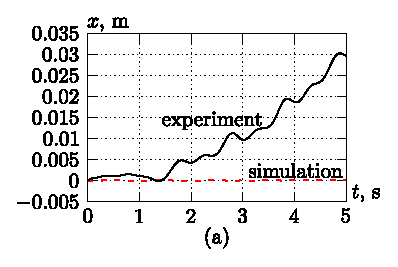
\includegraphics{id_x.eps}\hspace{20mm}\includegraphics{id_y.eps}
	\caption{Зависимости (a) $x(t)$ и (b) $y(t)$, полученные экспериментально и в результате моделирования на основе уравнений \eqref{eq.NE} с выражениями для сил и момента \eqref{eq.fgNS} и значениями коэффициентов \eqref{eq.coeffs1}} \label{fig.xy}
	%\textit{\textbf{Результаты моделирования}}
\end{figure}

\begin{figure}[h!]
	\centering
	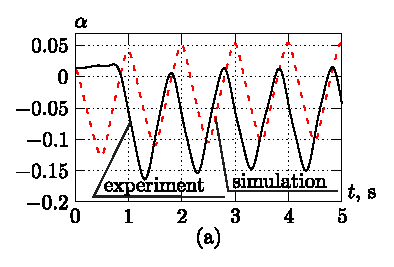
\includegraphics{id_phi.eps}\hspace{20mm}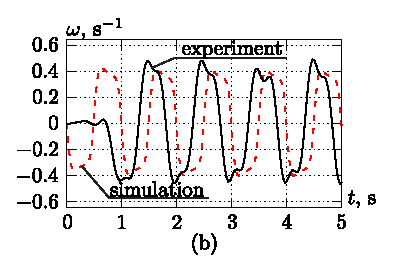
\includegraphics{id_omega.eps}
	\caption{Зависимости (a) $\alpha(t)$ и (b) $\omega(t)$, полученные экспериментально и в результате моделирования на основе уравнений \eqref{eq.NE} с выражениями для сил и момента \eqref{eq.fgNS} и значениями коэффициентов \eqref{eq.coeffs1}}\label{fig.phiOmega}
	%\textit{\textbf{Результаты моделирования}}
\end{figure}

Из рис. \ref{fig.xy}b видно, что предложенная модель воспроизводит колебания координаты $y$. Однако амплитуда колебаний $y$ в расчете меньше, чем в эксперименте. Из рис. \ref{fig.xy}a видно, что расчетные значения координаты $x$ на несколько порядков меньше по сравнению с экспериментальными. Из рис. \ref{fig.phiOmega} видно, что расчетные зависимости угла поворота $\alpha$ и угловой скорости $\omega$ согласуются с экспериментальными по частоте и амплитуде. Сдвиг по фазе на рис. \ref{fig.phiOmega} обусловлен тем, что на начальной стадии эксперимента имеется переходный процесс, отсутствующий при математическом моделировании. Таким образом, \textit{предложенная модель не воспроизводит самопродвижение робота со скоростью, наблюдаемой в эксперименте}.


\subsubsection*{Нестационарное обтекание}\label{ssec.unsteady}

%При достаточно продолжительном направленном движении твердого тела в жидкости происходит перераспределение сил давления по его поверхности и образуется пограничный слой. Это приводит к существенным изменениям значений сил и момента, действующих на тело. Поэтому в данном разделе будем определять коэффициенты, входящие в выражения \eqref{eq.forceTorque}, с использованием экспериментальных данных.

В предыдущем разделе было показано, что использование коэффициентов присоединенных масс, соответствующих чисто ускоренному движению, и коэффициентов сопротивления, соответствующих квазистационарному обтеканию, приводит к неудовлетворительным результатам. Поскольку движение робота является существенно нестационарным, оказывается невозможным определение коэффициентов $\lambda_{11}$, $\lambda_{22}$, $\lambda_{33}$, $\lambda_{23}$, $c_1$, $c_2$, $c_3$ по-отдельности. Таким образом данные коэффициенты должны определяться совместно с учетом нестационарности движение профиля.

Для задания граничных условий, соответствующих нестационарному движению профиля, будем использовать экспериментальные данные для прототипа, описанного в главе 5 с периодом управляющего воздействия $T = 1$ с, которые представляют собой таблицу значений:
\begin{gather}
	(t_i,\, x_i,\, y_i,\, \alpha_i),\quad i = 0,\, \ldots,\, N.\label{eq.expXYPhi}
\end{gather}
Здесь $t_i$ --- момент времени, $(x_i,\, y_i)$ --- положение центра масс профиля в момент времени $t_i$, $\alpha_i$ --- ориентация профиля в момент времени $t_i$.

Для определения поступательной и угловой скорости данные \eqref{eq.expXYPhi} были сглажены и продифференцированы методом Савицкого-Голая (Savitzky-Golay) \cite{Gorry_1990, Savitzky_Golay_1964}. Производные координат $\dot{x}_i$, $\dot{y}_i$ были пересчитаны в подвижную систему координат:
\begin{gather}
	v_{1,i} = \dot{x}_i \cos\alpha_i + \dot{y}_i \sin \alpha,\quad v_{2,i} = -\dot{x}_i \sin\alpha_i + \dot{y}_i \cos\alpha_i,\quad \omega_i = \dot{\alpha}_i.
\end{gather}
Выполняя дифференцирование табличных данных $v_{1,i}$, $v_{2,i}$, $\dot{\omega}_i$, получим ускорения:
\begin{gather}
	\dot{v}_{1,i},\quad \dot{v}_{2,i},\quad \dot{\omega}_i.
\end{gather}
Используя, табличные зависимости $v_1$, $v_2$, $\omega$ от времени, смоделируем движение робота и окружающей его жидкости. В результате расчета получим таблицу значений:
\begin{gather}
	(\dot{v}_{1,i},\, \dot{v}_{2,i},\, \dot{\omega}_i,\, v_{1,i},\, v_{2,i},\, \omega_i,\, f_{1,i},\, f_{2,i},\, g_i),\quad i = 1,\, \ldots,\, N.
\end{gather}

Согласно \eqref{eq.forceTorque} силы и момент зависят линейно от следующих величин:
\begin{gather}
	\dot{v}_{1},\quad \dot{v}_{2},\quad \dot{\omega},\quad
	v_{1} \omega,\quad v_{2} \omega,\quad v_{1}v_{2},\quad \omega^2,\quad v_1 |v_1|,\quad v_2 |v_2|,\quad \omega |\omega|.
\end{gather}
Это позволяет для вычисления коэффициентов присоединенных масс и коэффициентов сопротивления из результатов численного эксперимента применить метод наименьших квадратов. Кроме того, для лучшего согласования с экспериментальными данными в данном случае необходимо отказаться от требования симметрии коэффициентов (которое вытекает из модели идеальной жидкости). Окончательно получим следующие соотношения:
\begin{gather}
	\begin{gathered}
		f_1 = - \lambda_{11}^{(1)} \dot{v}_1 + \lambda_{22}^{(1)} v_2 \omega + \lambda_{23}^{(1)}\omega^2 - c_1 v_1 |v_1|, \\
		f_2 = - \lambda_{22}^{(2)} \dot{v}_2^{(2)} - \lambda_{23}^{(2)} \dot{\omega} - \lambda_{11}^{(2)} v_1 \omega - c_2 v_2 |v_2|,\\
		g = -\lambda_{23,l}^{(3)} \dot{v}_2 - \lambda_{33}^{(2)} \dot{\omega} + (\lambda_{11}^{(3)} - \lambda_{22}^{(3)}) v_1 v_2 - \lambda_{23,r}^{(3)} v_1\omega - c_3 \omega |\omega| - \dot{k}(t).
	\end{gathered}\label{eq.newfg}
\end{gather}


В результате обработки результатов моделирования (для управляющего воздействия с периодом $T = 1$ с) были получены следующие значения:
\begin{gather}
	\begin{gathered}
		\lambda_{11}^{(1)} \approx 0.3087, \quad 
		\lambda_{22}^{(1)} \approx -0.5796,\quad 
		\lambda_{23}^{(1)} \approx 0.039085,\\
		\lambda_{22}^{(2)} \approx 2.0996,\quad 
		\lambda_{23}^{(2)} \approx 0.17629,\quad
		\lambda_{11}^{(2)} \approx -7.9826,\\
		\lambda_{23,l}^{(3)} \approx 0.083474,\quad
		\lambda_{33}^{(2)} \approx 0.018935,\quad
		\lambda_{11}^{(3)} - \lambda_{22}^{(3)} \approx - 4.7550,\quad
		\lambda_{23,r}^{(3)} \approx 1.4488,\\
		c_1 = 0.04715,\quad c_2 = 17.702,\quad c_3 = 0.092872.
	\end{gathered}\label{eq.coeffs2}
\end{gather}


Результаты эксперимента и расчета с использованием коэффициентов \eqref{eq.coeffs2} представлены на рис. \ref{fig.xy1}, \ref{fig.phiOmega1}.

\begin{figure}[h!]
	\centering
	\includegraphics{visc_x.eps}\hspace{20mm}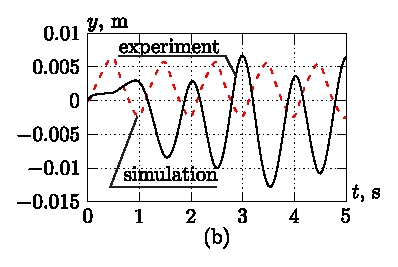
\includegraphics{visc_y.eps}
	\caption{Зависимости (a) $x(t)$ и (b) $y(t)$, полученные экспериментально и в результате моделирования на основе уравнений \eqref{eq.NE} с выражениями для сил и момента \eqref{eq.newfg} и значениями коэффициентов \eqref{eq.coeffs2}}\label{fig.xy1}
	%\textit{\textbf{Результаты моделирования}}
\end{figure}

\begin{figure}[h!]
	\centering
	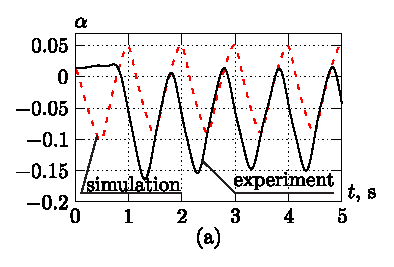
\includegraphics{visc_phi.eps}\hspace{20mm}\includegraphics{visc_omega.eps}
	\caption{Зависимости (a) $\alpha(t)$ и (b) $\omega(t)$, полученные экспериментально и в результате моделирования на основе уравнений \eqref{eq.NE} с выражениями для сил и момента \eqref{eq.newfg} и значениями коэффициентов \eqref{eq.coeffs2}}\label{fig.phiOmega1}
	%\textit{\textbf{Результаты моделирования}}
\end{figure}

Из рис. \ref{fig.xy1}, \ref{fig.phiOmega1} видно, что математическая модель \eqref{eq.NE} с силами и моментом \eqref{eq.newfg} и коэффициентами \eqref{eq.coeffs2} воспроизводит динамику рассматриваемой системы качественно и количественно. Таким образом, \textit{описанный в данном разделе метод определения коэффициентов математического модели обеспечивает лучшее согласование расчетных и экспериментальных данных}. Тем не менее, ниже будет показано, что в ряде случаев значения коэффициентов будут нуждаться в корректировке.



\section{Разработка и оценка алгоритма управления}



Анализ разработанной модели позволит сформировать управляющие воздействия. Из физических соображений очевидно, что чем более сложной и несимметричной является функция управления $\Omega(t)$, тем более сложную траекторию должен описывать робот. 

В экспериментах проводимых в работе~\cite{Pollard_Tallapragada_2016} для управления использовалась кусочно-постоянная по времени функция угловой скорости вращения ротора. Однако, на практике реализация такого кусочно-постоянного управления не возможна, из-за инерционности системы и ограниченности мощности приводного двигателя: он не может обеспечить мгновенное изменение угловой скорости вращения ротора, тем более со сменой направления вращения. В работе~\cite{Pollard_Tallapragada_2016} при вращении ротора по часовой и против часовой стрелки с равными угловыми скоростями и равными временными промежутками, робот плывет вдоль прямой. При неравенстве угловых скоростей вращения по часовой и против часовой стрелки, робот начинает двигаться вдоль окружности.

Учитывая временные промежутки вращения ротора с угловым ускорением зададим управление движением ротора $\Omega(t)$  при помощи кусочно-непрерывной периодической функции следующего вида:

\begin{gather}\label{omegaRotorGeneral}
\Omega(t) = \begin{cases}
\Omega_1(t), & t \in \left[ nT,\, nT + t_1 \right],\\
\Omega_2(t), & t \in \left[ nT + t_1,\, nT + t_1 + t_2 \right],\\
\Omega_3(t), & t \in \left[ nT + t_1 + t_2,\, nT + t_1 + t_2 + t_3 \right],\\
\Omega_4(t), & t \in \left[ nT + t_1 + t_2 + t_3,\, nT + t_1 + t_2 + t_3 + t_4 \right]
\end{cases}\\
\Omega_1(t) = \omega_1,\quad \Omega_2(t) = \dfrac{(\omega_2 - \omega_1)(t-nT)}{t_2} - \dfrac{(\omega_2 - \omega_1)(t_1+t_2)}{t_2} + \omega_2, \notag\\
\Omega_3(t) = \omega_2,\quad \Omega_4(t) = \dfrac{(\omega_1 - \omega_2)(t-nT)}{t_4} - \dfrac{(\omega_1 - \omega_2)(t_1+t_2+t_3+t_4)}{t_4} + \omega_1,\notag
\end{gather}
где $n \in \mathbb{N}$, $T$ --- период управляющего воздействия; $t_1, t_3$ --- задают интервалы времени с постоянными угловыми скоростями вращения ротора $\omega_1$, $\omega_2$ соответственно, $t_2$, $t_4$ --- интервалы равноускоренного вращения ротора. Графически данная зависимость приведена на рис.~\ref{ControlAction}.

\begin{figure}[!ht]
	\centering
	\includegraphics[width=0.4\linewidth]{ControlAction.eps}
	\caption{График зависимости угловой скорости вращения ротора от времени в общем виде}
	\label{ControlAction}
\end{figure}

Мы видим, что простейшее управление вида \eqref{omegaRotorGeneral} позволяет учесть два типа асимметрии, во-первых, сдвиг $ \Omega(t) \rightarrow \omega_0 + \Omega(t) $,
%\begin{gather}
%\Omega(t) \rightarrow \omega_0 + \Omega(t),
%\end{gather}
во-вторых, неравенство ускорений за время одного периода управляющего воздействия.

Анализируя соотношения \eqref{eq.forceTorque}, видно, что уравнения движения содержат не угловую скорость ротора, а только его ускорение $\dot{\Omega}(t)$. Отсюда следует, что данная модель предполагает, в частности, что форма траектории робота не должна зависеть от сдвига $\omega_0$, что противоречит результатам работы~\cite{Pollard_Tallapragada_2016}. Проверим насколько это согласуется с экспериментом.

Заметим, что на практике обеспечить промежутки $t_2$ и $t_4$ сколь угодно малыми невозможно. Это обусловлено инерцией ротора и ограниченностью мощности приводного двигателя, вследствие чего он не может обеспечить мгновенное изменение угловой скорости вращения ротора, тем более со сменой направления вращения.

В следующей главе рассмотрим результаты численного моделирования и экспериментальных исследований при различных соотношениях угловых скоростей вращения ротора $\omega_1$, $\omega_2$, а также длительностей интервалов $t_1$, $t_2$, $t_3$, $t_4$.


\section{Исследование уравнений движения}

Управляющее воздействие (\ref{omegaRotorGeneral}) может принимать различную форму. Рассмотрим случаи с управляющим воздействием симметричным на периоде и ассиметричным. %Во всех случаях моделирования период управляющего воздействия зададим равным $T=5$ секунд. 


\subsection{Исследование зависимости формы траектории от характера управляющего воздействия}



\textbf{Управляющее воздействие симметричное на периоде.} Для обеспечения симметричности должны выполняться условия: $t_1=t_3$, $t_2=t_4$. Проведем моделирование движения робота при $t_1=t_3=2$ с., $t_2=t_4 = 0.5$ с. Время моделирования -- 50 секунд. Рассчитанная траектория движения представлена на рисунке~\ref{xyModelLine1}.

\begin{figure}[!ht]
	\centering
	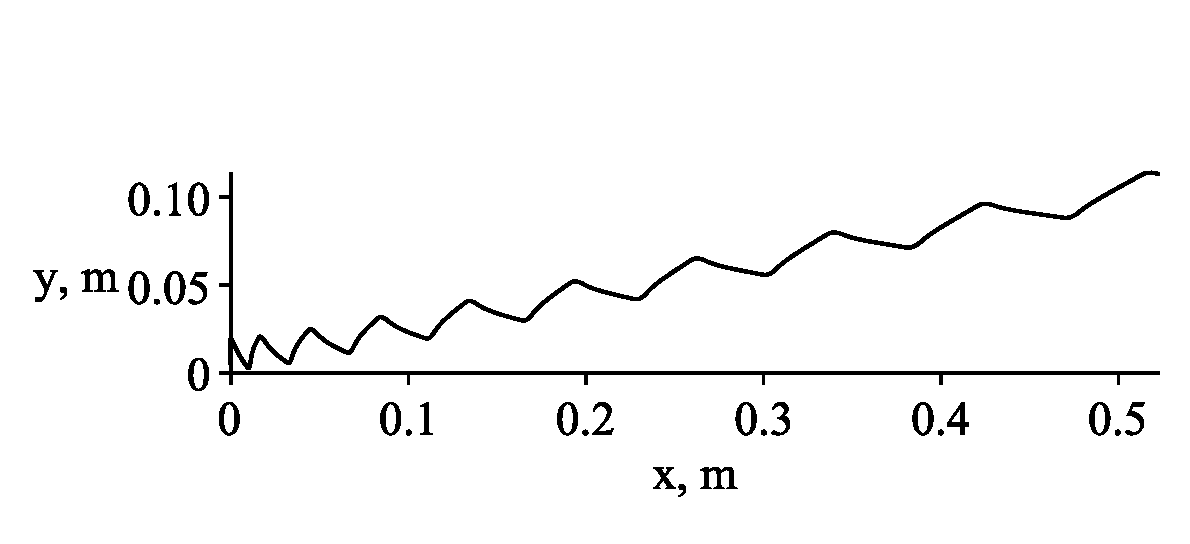
\includegraphics[width=0.7\linewidth]{xyModelLine1.eps}
	\caption{Траектория движения робота}
	\label{xyModelLine1}
\end{figure}

\textbf{Управляющее воздействие асимметричное на периоде.} Рассмотрим первый случай, когда участки равноускоренного движения ротора равны, а участки вращения с постоянной скоростью не равны --- $t_1 \neq t_3$, $t_2=t_4$. Проведем моделирование движения робота при $t_1=1$ c., $t_3=3$ с., $t_2=t_4 = 0.5$ с. Время моделирования -- 200 секунд. Рассчитанная траектория движения представлена на рисунке~\ref{xyModelCircle1}.

\begin{figure}[!ht]
	\centering
	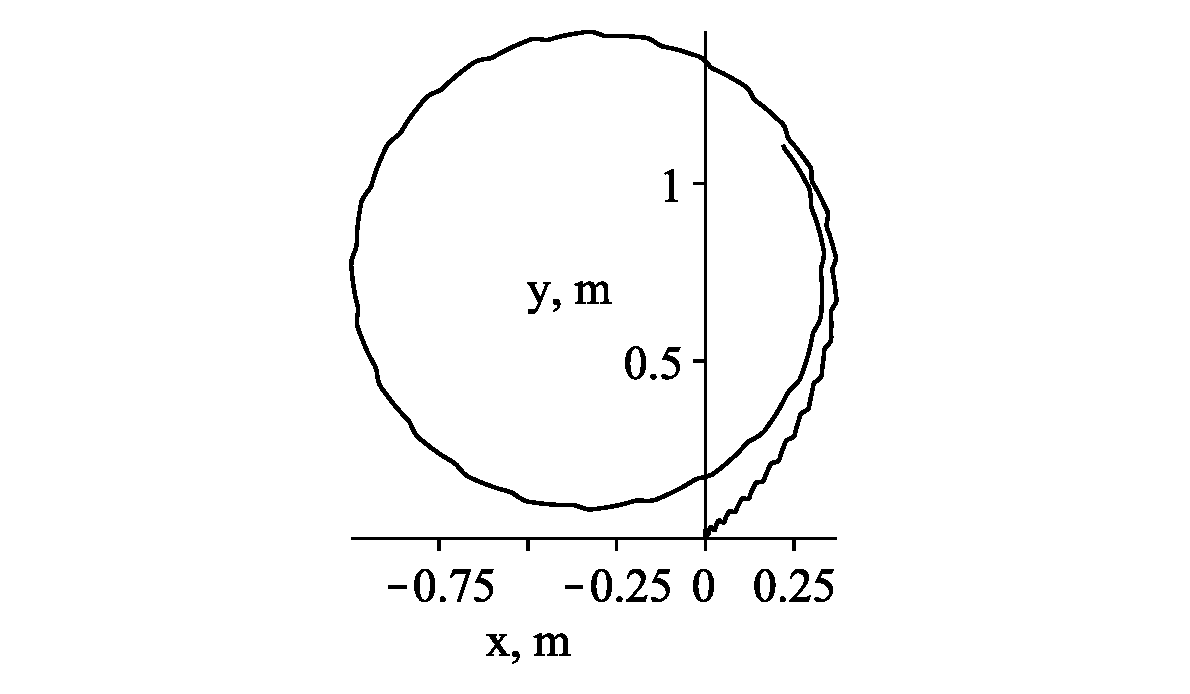
\includegraphics[width=0.7\linewidth]{xyModelCircle1.eps}
	\caption{Траектория движения робота}
	\label{xyModelCircle1}
\end{figure}

Рассмотрим второй случай с равными по времени участками вращения ротора с постоянной скоростью --- $t_1 = t_3$, и не равными по времени участками равноускоренного вращения ротора $t_2 \neq t_4$. Проведем моделирование движения робота при $t_1=t_3=1$ с., $t_2=0.5$ с. $t_4 = 2.5$ с. Время моделирования -- 200 секунд. Рассчитанная траектория движения представлена на рисунке~\ref{xyModelCircle2}.

\begin{figure}[!ht]
	\centering
	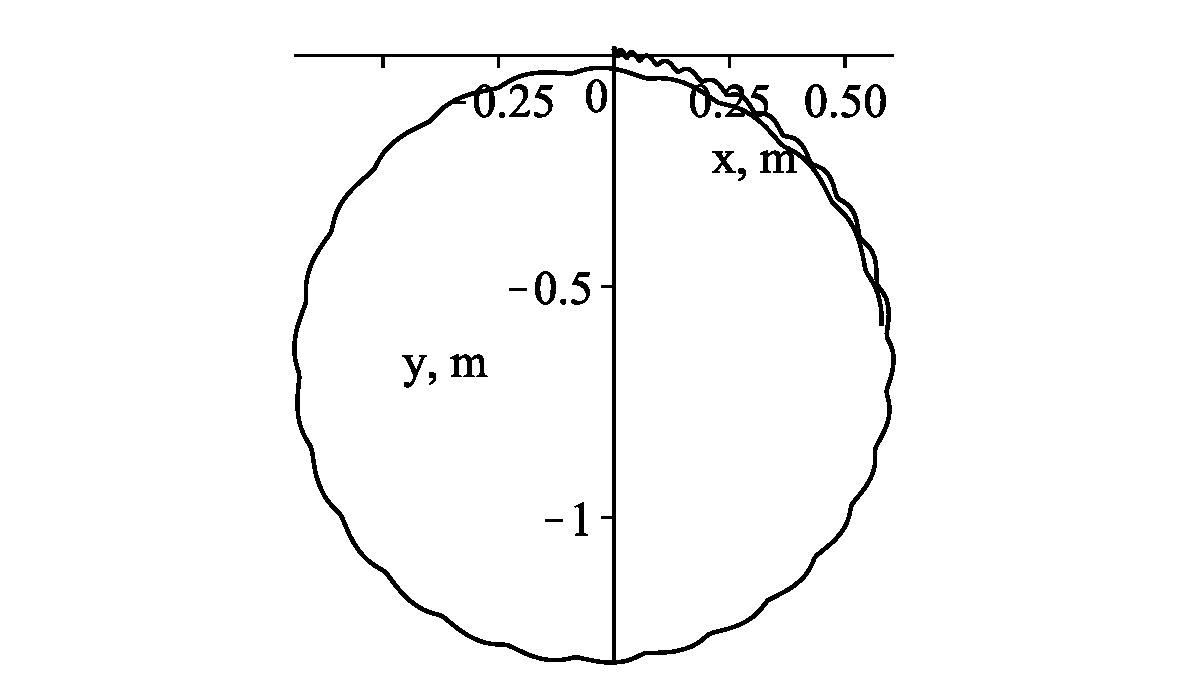
\includegraphics[width=0.7\linewidth]{xyModelCircle2.eps}
	\caption{Траектория движения робота}
	\label{xyModelCircle2}
\end{figure}

Рассмотрим третий случай с не равными по времени участками вращения ротора с постоянной скоростью --- $t_1 \neq t_3$, и не равными по времени участками равноускоренного вращения ротора $t_2 \neq t_4$. Проведем моделирование движения робота при $t_1=1$ с., $t_3=2$ с., $t_2=0.5$ с. $t_4 = 1.5$ с. Время моделирования -- 200 секунд. Рассчитанная траектория движения представлена на рисунке~\ref{xyModelCircle3}.

\begin{figure}[!ht]
	\centering
	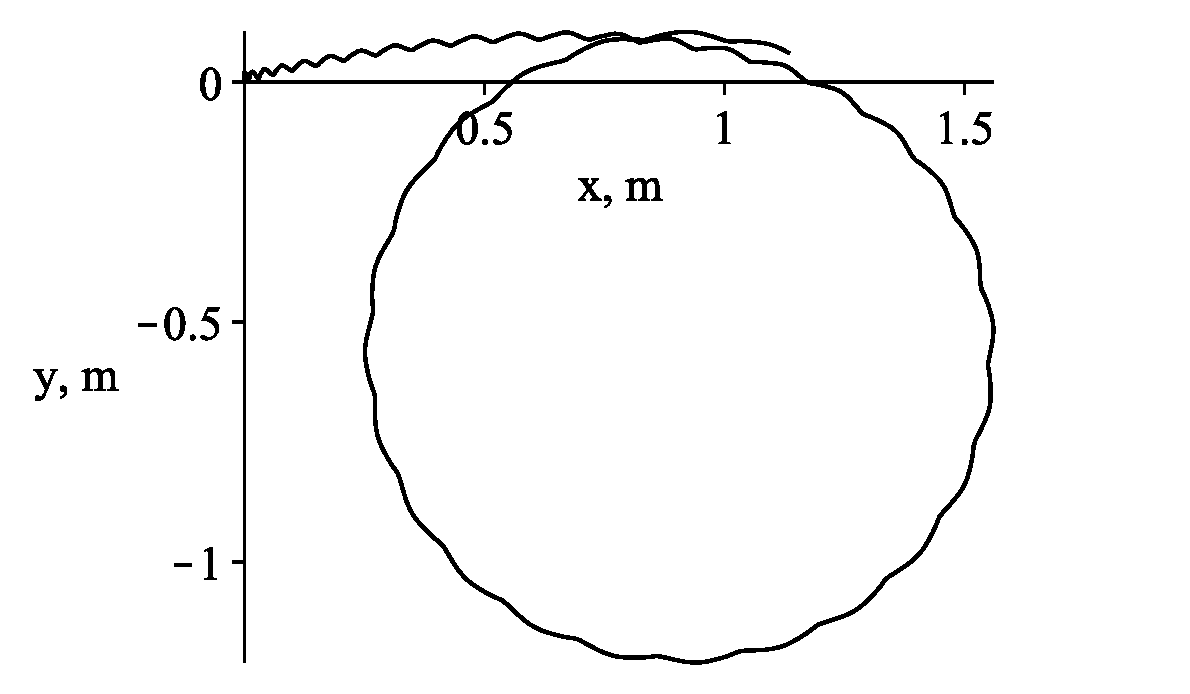
\includegraphics[width=0.7\linewidth]{xyModelCircle3.eps}
	\caption{Траектория движения робота}
	\label{xyModelCircle3}
\end{figure}

\textbf{Управляющее воздействие с различной амплитудой угловой скорости ротора.} Рассмотрим симметричное управляющее воздействие при $t_1=t_3=2$ с., $t_2=t_4 = 0.5$ с., но с разной амплитудой скоростей $\omega_1$ и $\omega_2$.  На рисунке~\ref{xyModelLineDifferentW} представлены три рассчитанные траектории движения робота: черная линия -- $\omega_1=10$ рад/с и $\omega_2=-10$ рад/с; красная линия -- $\omega_1=10$ рад/с и $\omega_2=-3$ рад/с; синяя линия -- $\omega_1=10$ рад/с и $\omega_2=3$ рад/с. Время моделирования -- 50 секунд.

\begin{figure}[!ht]
	\centering
	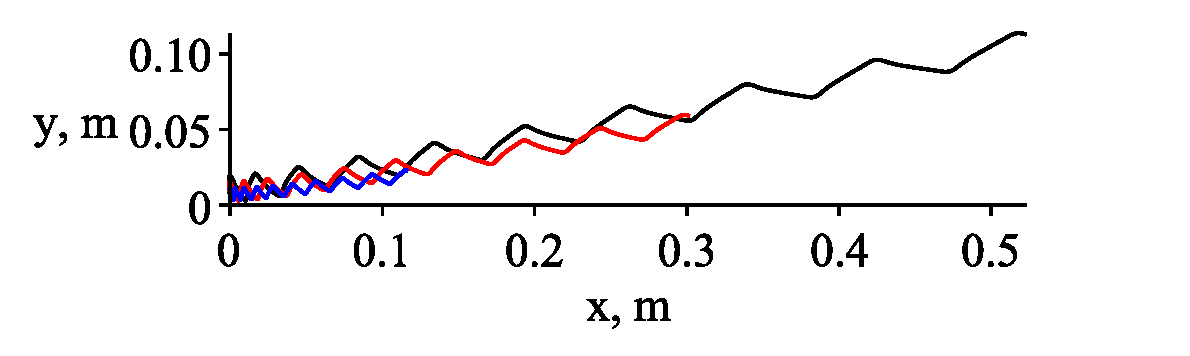
\includegraphics[width=0.7\linewidth]{xyModelLineDifferentW.eps}
	\caption{Траектория движения робота}
	\label{xyModelLineDifferentW}
\end{figure}

Рассмотрим также асимметричное управляющее воздействие при $t_1=3$ с., $t_3=1$ с., $t_2=t_4 = 0.5$ с., но с разной амплитудой скоростей $\omega_1$ и $\omega_2$. На рисунке~\ref{xyModelCircleDifferentW}, аналогично моделированию с симметричным управляющим воздействием, представлены три рассчитанные траектории движения робота: черная линия -- $\omega_1=10$ рад/с и $\omega_2=-10$ рад/с; красная линия -- $\omega_1=10$ рад/с и $\omega_2=-3$ рад/с; синяя линия -- $\omega_1=10$ рад/с и $\omega_2=3$ рад/с. Время моделирования -- 200 секунд.

\begin{figure}[!ht]
	\centering
	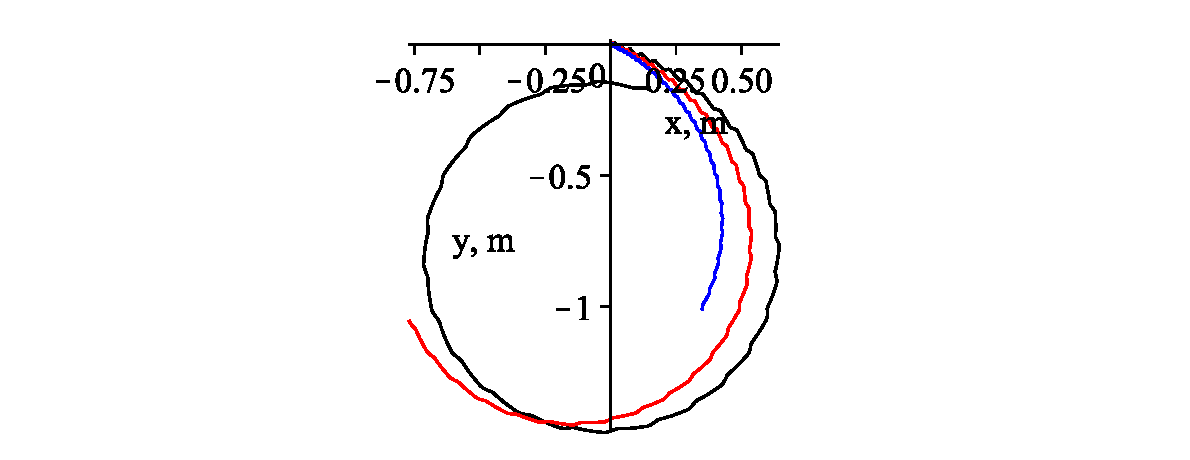
\includegraphics[width=0.8\linewidth]{xyModelCircleDifferentW.eps}
	\caption{Траектория движения робота}
	\label{xyModelCircleDifferentW}
\end{figure}

\textbf{Управляющее воздействие со смещением амплитуды угловой скорости ротора.} Рассмотрим симметричное управляющее воздействие при $t_1=t_3=2$ с., $t_2=t_4 = 0.5$ с., но со смещением амплитуды угловых скоростей $\omega_1$ и $\omega_2$ при этом $\omega_1 - \omega_2 = const$.  На рисунке~\ref{xyModelLineDifferentW2} представлена рассчитанная траектория движения робота, соответствующая трем различным управляющим воздействиям: 1: $\omega_1=10$ рад/с и $\omega_2=-3$ рад/с; 2: $\omega_1=6.5$ рад/с и $\omega_2=-6.5$ рад/с; 3: $\omega_1=3$ рад/с и $\omega_2=-10$ рад/с. Время моделирования -- 50 секунд.

\begin{figure}[!ht]
	\centering
	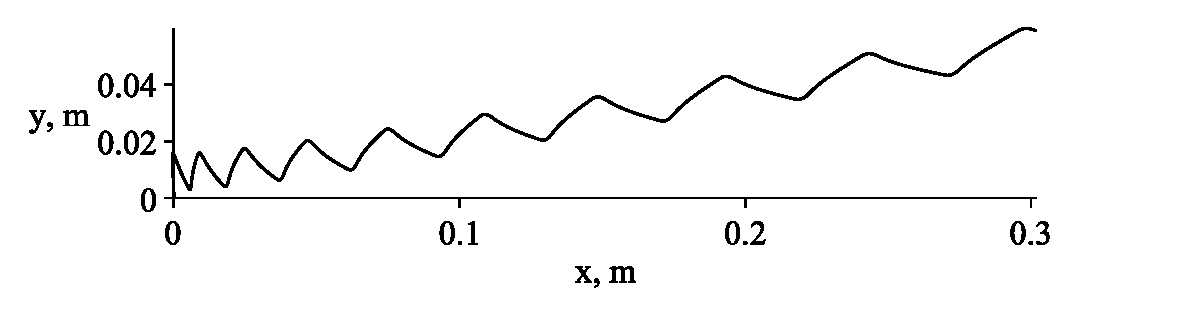
\includegraphics[width=0.7\linewidth]{xyModelLineDifferentW2.eps}
	\caption{Траектория движения робота}
	\label{xyModelLineDifferentW2}
\end{figure}

Для асимметричного управляющего воздействия смещение амплитуды угловой скорости ротора также на форму траектории не влияет. Рассмотрим моделирование при $t_1=3$ с., $t_3=1$ с., $t_2=t_4 = 0.5$ с., и с амплитудой скоростей $\omega_1 - \omega_2 = const$. На рисунке~\ref{xyModelCircleDifferentW2} представлена рассчитанная траектория движения робота, соответствующая трем различным управляющим воздействиям: 1: $\omega_1=10$ рад/с и $\omega_2=-3$ рад/с; 2: $\omega_1=6.5$ рад/с и $\omega_2=-6.5$ рад/с; 3: $\omega_1=3$ рад/с и $\omega_2=-10$ рад/с. Время моделирования -- 200 секунд.

\begin{figure}[!ht]
	\centering
	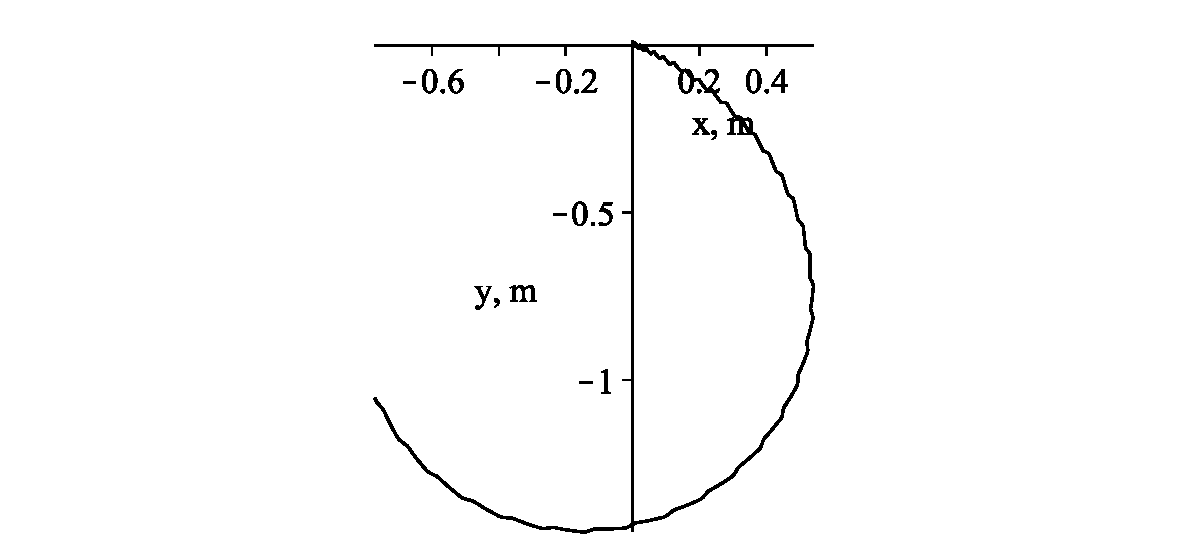
\includegraphics[width=0.7\linewidth]{xyModelCircleDifferentW2.eps}
	\caption{Траектория движения робота}
	\label{xyModelCircleDifferentW2}
\end{figure}

\textbf{Выводы.} Как видно из моделирования, при симметричном на периоде управляющем воздействии робот движется в среднем по прямой. При ассиметричном на периоде управляющем воздействии робот движется по траектории близкой к окружности при различных случаях ассиметрии. В рассмотренных трех случаях ассиметрии управляющего воздействия радиус окружности траектории движения практически не изменяется, изменяется направление движения в начальный момент времени.

При прочих равных условиях амплитуда угловой скорости ротора $\omega_1 - \omega_2$ влияет на величину пройденного пути по траектории, поэтому максимальный эффект от движения недеформируемого водного робота с острой кромкой наблюдается при максимальной амплитуде угловой скорости ротора $\omega_1 - \omega_2 = 2\omega_{max}$.

При постоянном значении амплитуды угловой скорости ротора $\omega_1 - \omega_2 = const$ при прочих равных условиях форма траектории не изменяется при любых $\omega_1$ и $\omega_2$.


\subsection{Исследование зависимости формы траектории от параметров модели}

\textbf{Момент инерции ротора.} Проверим как влияет величина момента инерции ротора на траекторию движения. Рассмотрим движение вдоль прямой при симметричном управляющем воздействии с параметрами $t_1=t_3=2$ с., $t_2=t_4 = 0.5$ с., $\omega_1=10$ рад/с, $\omega_2=-10$ рад/с. Проведем моделирование с тремя значениями момента инерции ротора: $I_r = 0.00058$ кг$\cdot$м$^2$ -- реальное значение момента инерции ротора; $I_r = 0.00116$ кг$\cdot$м$^2$ -- удвоенное значение момента инерции ротора; $I_r = 0.00029$ кг$\cdot$м$^2$ -- половина от реального значения момента инерции ротора. На рисунке~\ref{xyModelInertion} представлены рассчитанные траектории движения робота при различных значениях момента инерции ротора: черная линия --- $I_r = 0.00116$ кг$\cdot$м$^2$; красная линия --- $I_r = 0.00058$ кг$\cdot$м$^2$; синяя линия --- $I_r = 0.00029$ кг$\cdot$м$^2$. Время моделирования -- 50 секунд.

\begin{figure}[!ht]
	\centering
	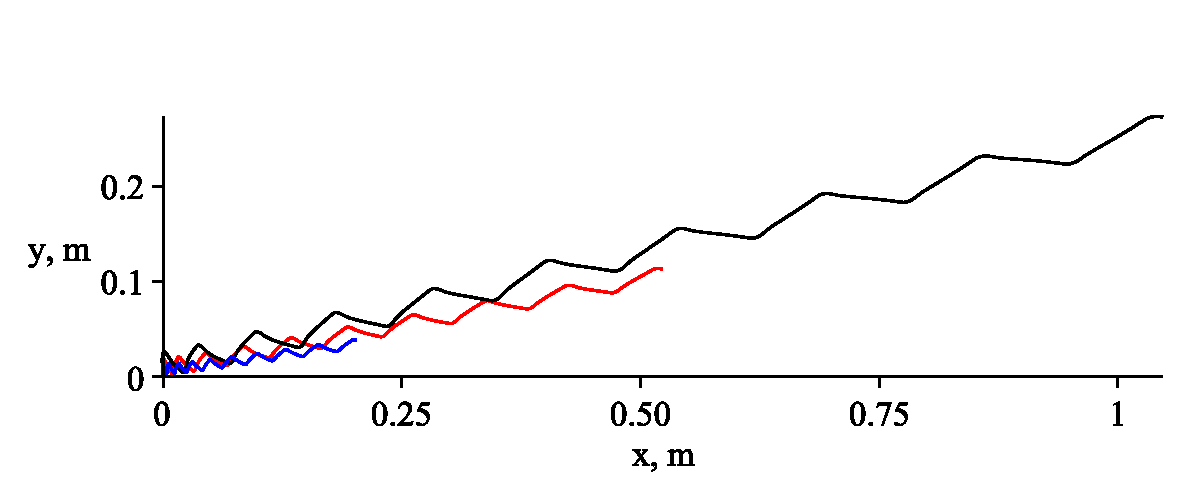
\includegraphics[width=0.7\linewidth]{xyModelInertion.eps}
	\caption{Траектория движения робота}
	\label{xyModelInertion}
\end{figure}

\textbf{Масса ротора.} Далее проверим влияние массы ротора на траекторию движения. Рассмотрим движение вдоль прямой при симметричном управляющем воздействии с параметарми $t_1=t_3=2$ с., $t_2=t_4 = 0.5$ с., $\omega_1=10$ рад/с, $\omega_2=-10$ рад/с. Проведем моделирование с тремя значениями массы ротора: $m_r = 0.327$ кг -- реальное значение массы ротора; $m_r = 0.654$ кг -- удвоенное значение массы ротора; $m_r = 0.163$ кг -- половина от реального значения массы ротора. На рисунке~\ref{xyModelMass} представлены рассчитанные траектории движения робота при различных значениях массы ротора: черная линия --- $m_r = 0.654$ кг; красная линия --- $m_r = 0.327$ кг; синяя линия --- $m_r = 0.1635$ кг. Время моделирования -- 50 секунд.

\begin{figure}[!ht]
	\centering
	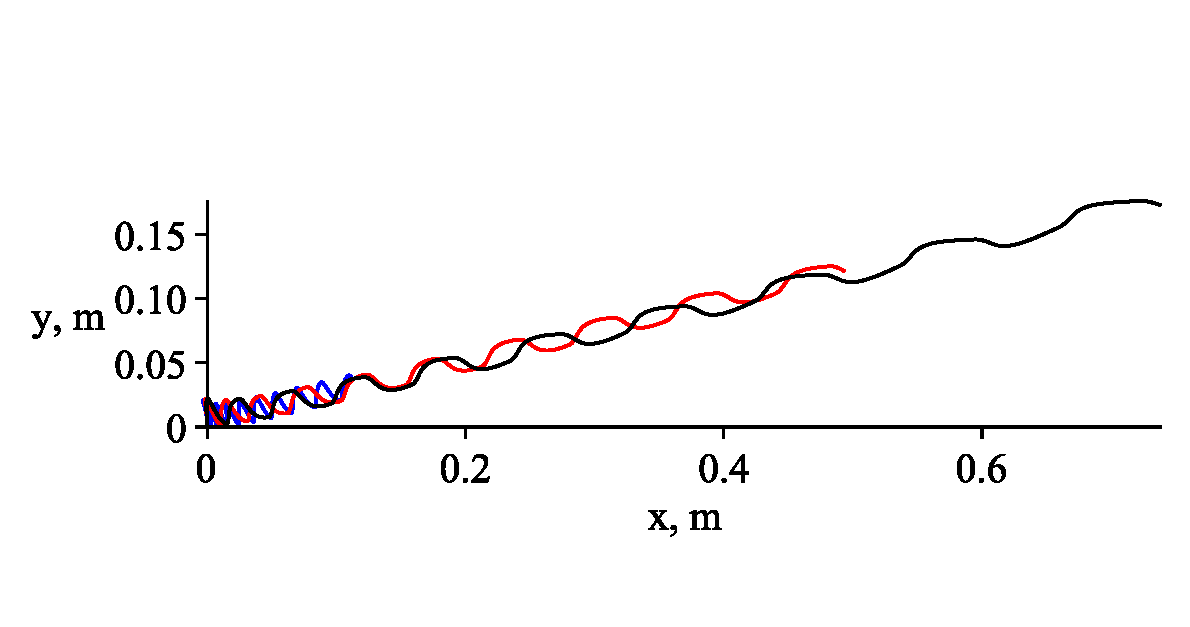
\includegraphics[width=0.7\linewidth]{xyModelMass.eps}
	\caption{Траектория движения робота}
	\label{xyModelMass}
\end{figure}

\textbf{Расположение ротора.} Далее проверим влияние расположения ротора на траекторию движения. Рассмотрим движение вдоль прямой при симметричном управляющем воздействии с параметарми $t_1=t_3=2$ с., $t_2=t_4 = 0.5$ с., $\omega_1=10$ рад/с, $\omega_2=-10$ рад/с. Проведем моделирование с тремя значениями смещения ротора относительно центра масс системы: $\xi_r = 0$ -- смещение ротора отсутствует; $\xi_r = 0.1$ м; $\xi_r = 0.2$ м. На рисунке~\ref{xyModelCenterOfMass} представлены рассчитанные траектории движения робота при различных значениях смещения центра масс ротора относительно центра масс системы: черная линия --- $\xi_r = 0$ -- смещение отсутствует; красная линия ---  $\xi_r = 0.1$ м; синяя линия --- $\xi_r = 0.2$ м. Время моделирования -- 50 секунд.

\begin{figure}[!ht]
	\centering
	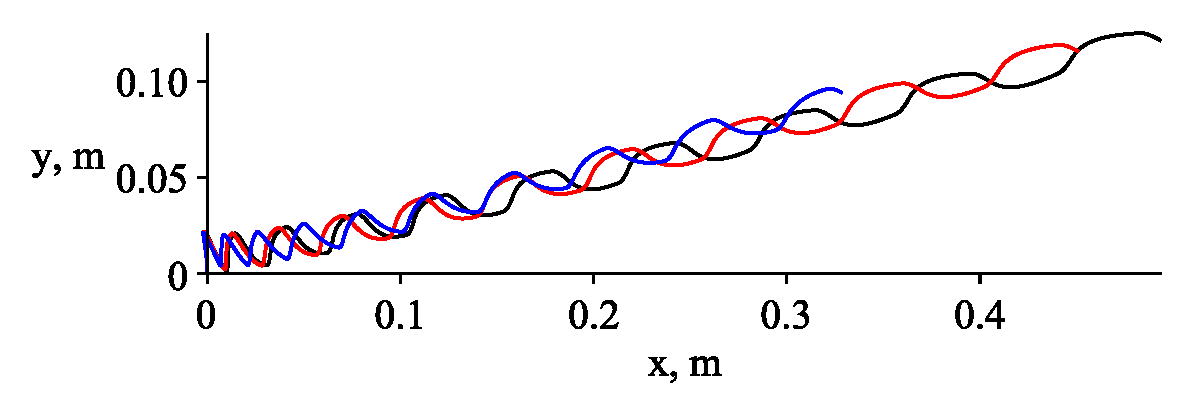
\includegraphics[width=0.7\linewidth]{xyModelCenterOfMass.eps}
	\caption{Траектория движения робота}
	\label{xyModelCenterOfMass}
\end{figure}

\textbf{Выводы.} Из графиков видно, что при увеличении вдвое момента инерции ротора, пройденное расстояние увеличивается также вдвое. Однако при увеличении массы ротора пройденное расстояние уменьшается пропорционально изменению массы всего робота (масса оболочки + масса ротора). Наибольший эффект достигается при расположении ротора в центре масс системы. Поэтому для эффективного движения необходимо использовать ротор с максимально возможным моментом инерции и минимальной массой расположенный в центре масс всей системы.

Осевой момент инерции тела рассчитывается как сумма произведений масс всех $n$ материальных точек системы на квадраты их расстояний до оси: $I = \sum \limits_{i=1}^n m_i\cdot r_i^2$. Осевой момент инерции тела зависит от массы линейно, а от радиуса -- квадратично. Поэтому если сосредоточить основную массу ротора на наиболее удаленном расстоянии от оси вращения можно добиться максимального момента инерции при минимальной массе. Диаметр ротора ограничен оболочкой робота и для данной модели максимальный радиус ротора 110 мм.


%3Д-модель ротора, удовлетворяющего вышеописанным требованиям представлена на рисунке~\ref{RotorNACA}.


%\begin{figure}[!ht]
%	\centering
%	\includegraphics[width=0.5\linewidth]{RotorNACA.png}
%	\caption{3Д-модель ротора с максимальным моментом инерции при минимальной массе}
%	\label{RotorNACA}
%\end{figure}


\section{Выводы по главе}

В данной главе разработана математическая модель движения недеформируемого водного робота с острой кромкой за счет вращения внутреннего ротора для движения по поверхности жидкости с учетом действия вязких сил. Разработан алгоритм управления роботом, представлен вид функции управления в виде изменения угловой скорости ротора во времени. По разработанным модели движения и алгоритму управления поведены исследования зависимости фомры траектории от характера управляющего воздействия и от параметров прототипа робота. Получены формы управляющих воздействий для движения вдоль прямой и вдоль окружности. Показано, что для наиболее эффективного движения необходимо использовать ротор с максимально возможным моментом инерции при наименьшей массе, который расположен в центре масс системы.


\clearpage